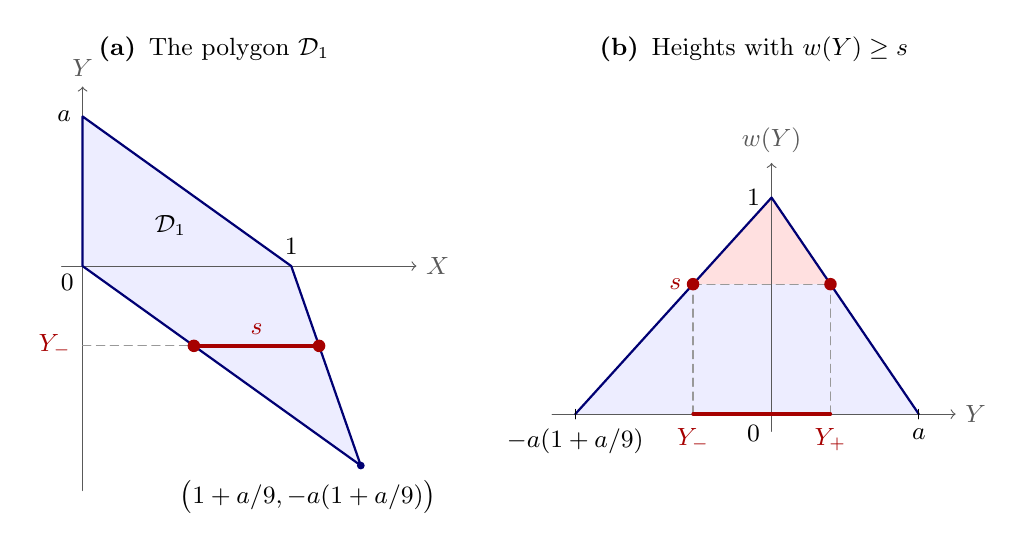
\begin{tikzpicture}[
  font=\small,
  line cap=round,
  line join=round,
  axis/.style={->,thin,black!65},
  boundary/.style={thick,blue!45!black},
  guide/.style={densely dashed,thin,black!40},
  sample/.style={very thick,red!65!black},
  slicepoint/.style={circle,inner sep=1.6pt,fill=red!65!black}
]
  \begin{scope}[x=2.65cm,y=1.90cm]
    \node[anchor=south] at (.63,1.30)
      {\textbf{(a)}\enspace The polygon $\mathcal D_1$};
    \fill[blue!7] (0,0)--(0,1)--(1,0)--(4/3,-4/3)--cycle;
    \draw[axis] (-.10,0)--(1.60,0) node[right] {$X$};
    \draw[axis] (0,-1.50)--(0,1.20) node[above] {$Y$};
    \draw[boundary] (0,0)--(0,1)--(1,0)--(4/3,-4/3)--cycle;
    \node[anchor=south west] at (.30,.14) {$\mathcal D_1$};
    \node[anchor=north east,inner sep=3pt] at (0,0) {$0$};
    \node[anchor=east,inner sep=4pt] at (0,1) {$a$};
    \node[anchor=south,inner sep=4pt] at (1,0) {$1$};
    \draw[guide] (0,-8/15)--(8/15,-8/15);
    \draw[sample] (8/15,-8/15)--(17/15,-8/15);
    \node[slicepoint] at (8/15,-8/15) {};
    \node[slicepoint] at (17/15,-8/15) {};
    \node[anchor=east,inner sep=4pt,text=red!65!black]
      at (0,-8/15) {$Y_-$};
    \node[anchor=south,inner sep=4pt,text=red!65!black]
      at (5/6,-8/15) {$s$};
    \fill[blue!45!black] (4/3,-4/3) circle (1.4pt);
    \node[anchor=north,inner sep=5pt] at (1.08,-4/3)
      {$\bigl(1+a/9,-a(1+a/9)\bigr)$};
  \end{scope}

  \begin{scope}[shift={(8.75cm,-1.88cm)},x=1.87cm,y=2.75cm]
    \node[anchor=south] at (-.12,1.58)
      {\textbf{(b)}\enspace Heights with $w(Y)\ge s$};
    \fill[blue!7] (-4/3,0)--(0,1)--(1,0)--cycle;
    \fill[red!12] (-8/15,3/5)--(0,1)--(2/5,3/5)--cycle;
    \draw[axis] (-1.49,0)--(1.25,0) node[right] {$Y$};
    \draw[axis] (0,-.08)--(0,1.16) node[above] {$w(Y)$};
    \draw[boundary] (-4/3,0)--(0,1)--(1,0);
    \draw[guide] (-8/15,0)--(-8/15,3/5);
    \draw[guide] (2/5,0)--(2/5,3/5);
    \draw[guide] (-8/15,3/5)--(2/5,3/5);
    \draw[sample] (-8/15,0)--(2/5,0);
    \node[slicepoint] at (-8/15,3/5) {};
    \node[slicepoint] at (2/5,3/5) {};
    \draw[thin] (-4/3,.022)--(-4/3,-.022);
    \draw[thin] (1,.022)--(1,-.022);
    \node[anchor=north,inner sep=5pt] at (-4/3,0)
      {$-a(1+a/9)$};
    \node[anchor=north,inner sep=5pt] at (1,0) {$a$};
    \node[anchor=north east,inner sep=4pt] at (0,0) {$0$};
    \node[anchor=east,inner sep=4pt] at (0,1) {$1$};
    \node[anchor=north,inner sep=5pt,text=red!65!black]
      at (-8/15,0) {$Y_-$};
    \node[anchor=north,inner sep=5pt,text=red!65!black]
      at (2/5,0) {$Y_+$};
    \node[anchor=east,inner sep=4pt,text=red!65!black]
      at (-8/15,3/5) {$s$};
  \end{scope}
\end{tikzpicture}
